\section{Week 8: 9th - 15th March 2026}

\subsection{Tuesday 10th March}

\begin{itemize}
    \item My main issue with the GPR fitting was that something wasn't working with modelling the foreground signal properly and the signal wasn't getting cleaned.
    \item A suggestion was that instead of finding the best optimisation method, try different kernels to see if those work better.
    \item I had another look at the main GPR papers and looked at different kernels I could model.
    \item I wrote new functions for the matern kernel with different eta values and then the rbf kernel without the spectral parameter (where before I was fitting the rbf kernel with the spectral parameter).
    \item An issue I also had with GPR is that the length scale for foreground almost always hit the upper bounds. I had the thought to run the parameter optimisation but fix the foreground length scale so that it does not hit the upper bounds.
\end{itemize}

\clearpage

\subsubsection{Scipy optimize minimize, Nelder-Mead, RBF kernel without spectral index}

\begin{figure}[htb!]
    \centering
    \begin{minipage}{0.49\textwidth}
        \centering
        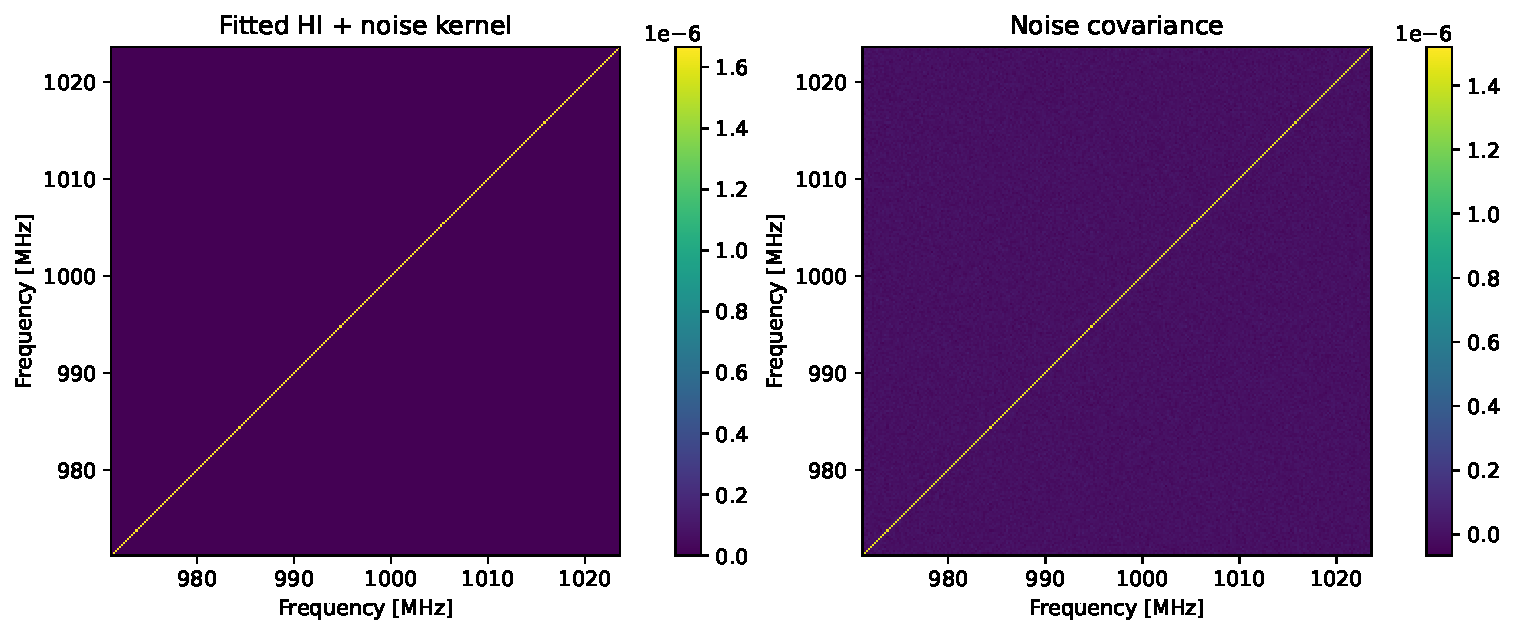
\includegraphics[width=\linewidth]{outputs/week8/hi_signal_kernal_comparison_fixed_l_fg_no_sp_indx.pdf}
        \label{fig:pspec_lin_0_01}
    \end{minipage}
    \hfill
    \begin{minipage}{0.49\textwidth}
        \centering
        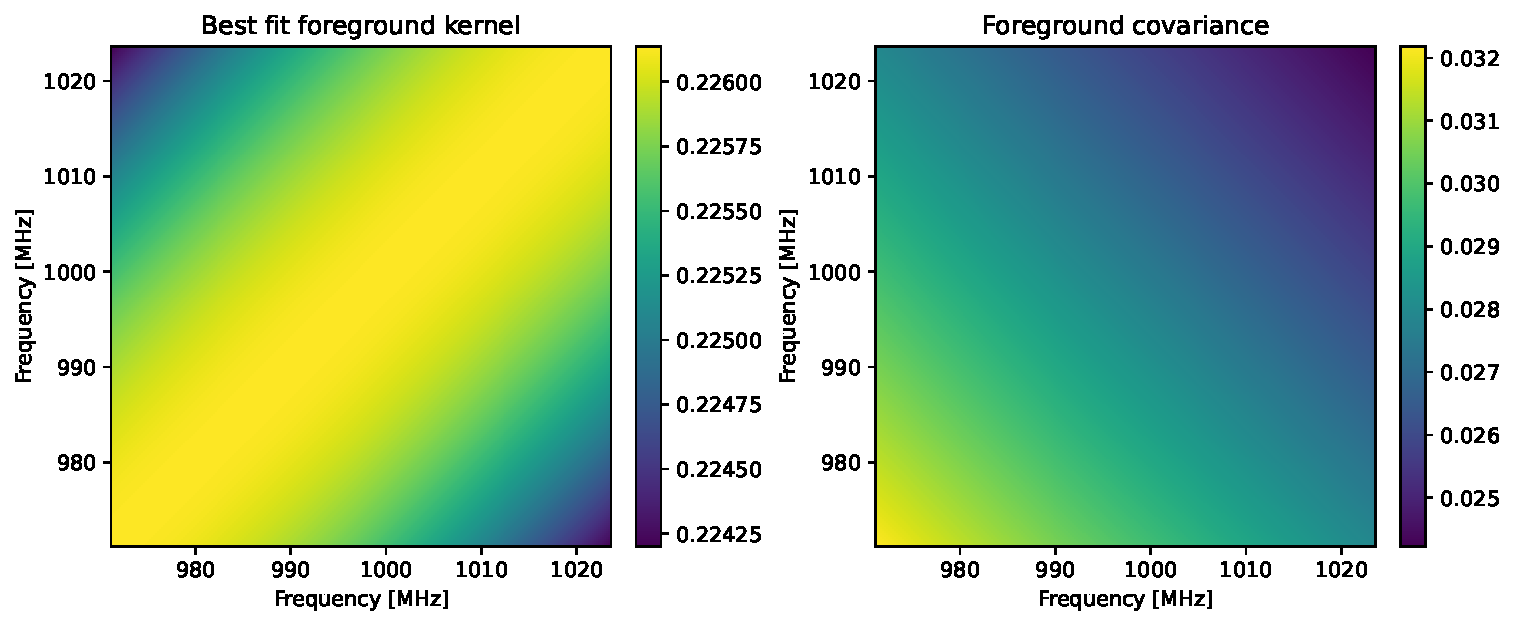
\includegraphics[width=\linewidth]{outputs/week8/fg_signal_kernal_comparison_fixed_l_fg_no_sp_indx.pdf}
        \label{fig:pspec_log_0_01}
    \end{minipage}
    \caption{Enter Caption}
\end{figure}

\begin{figure}[hbt!]
    \centering
    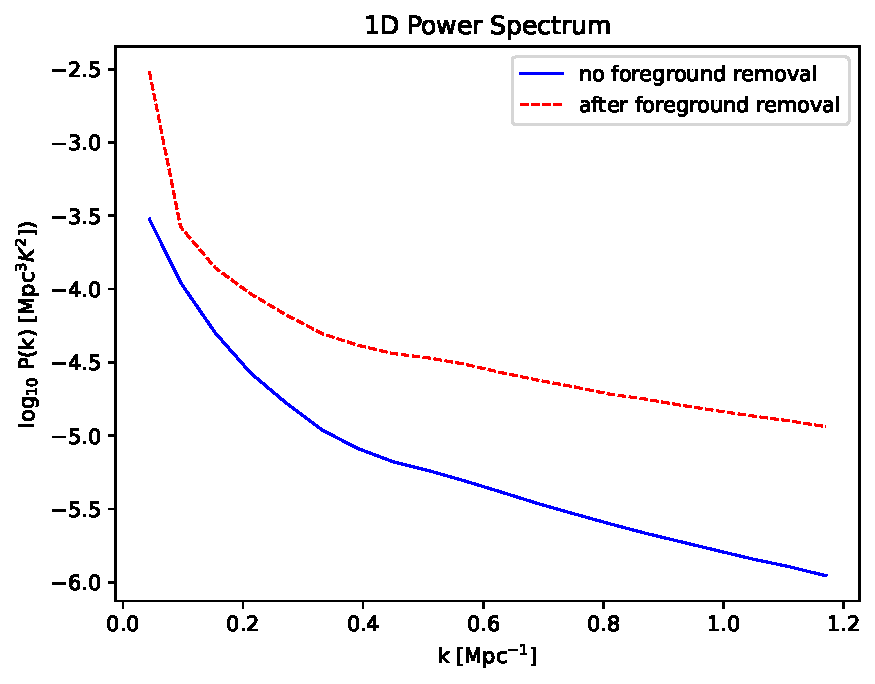
\includegraphics[width=0.4\linewidth]{outputs/week8/log_1d_power_spectrum_fixed_l_fg_no_sp_indx.pdf}
    \caption{Enter Caption}
    \label{fig:placeholder}
\end{figure}

\begin{figure}[hbt!]
    \centering
    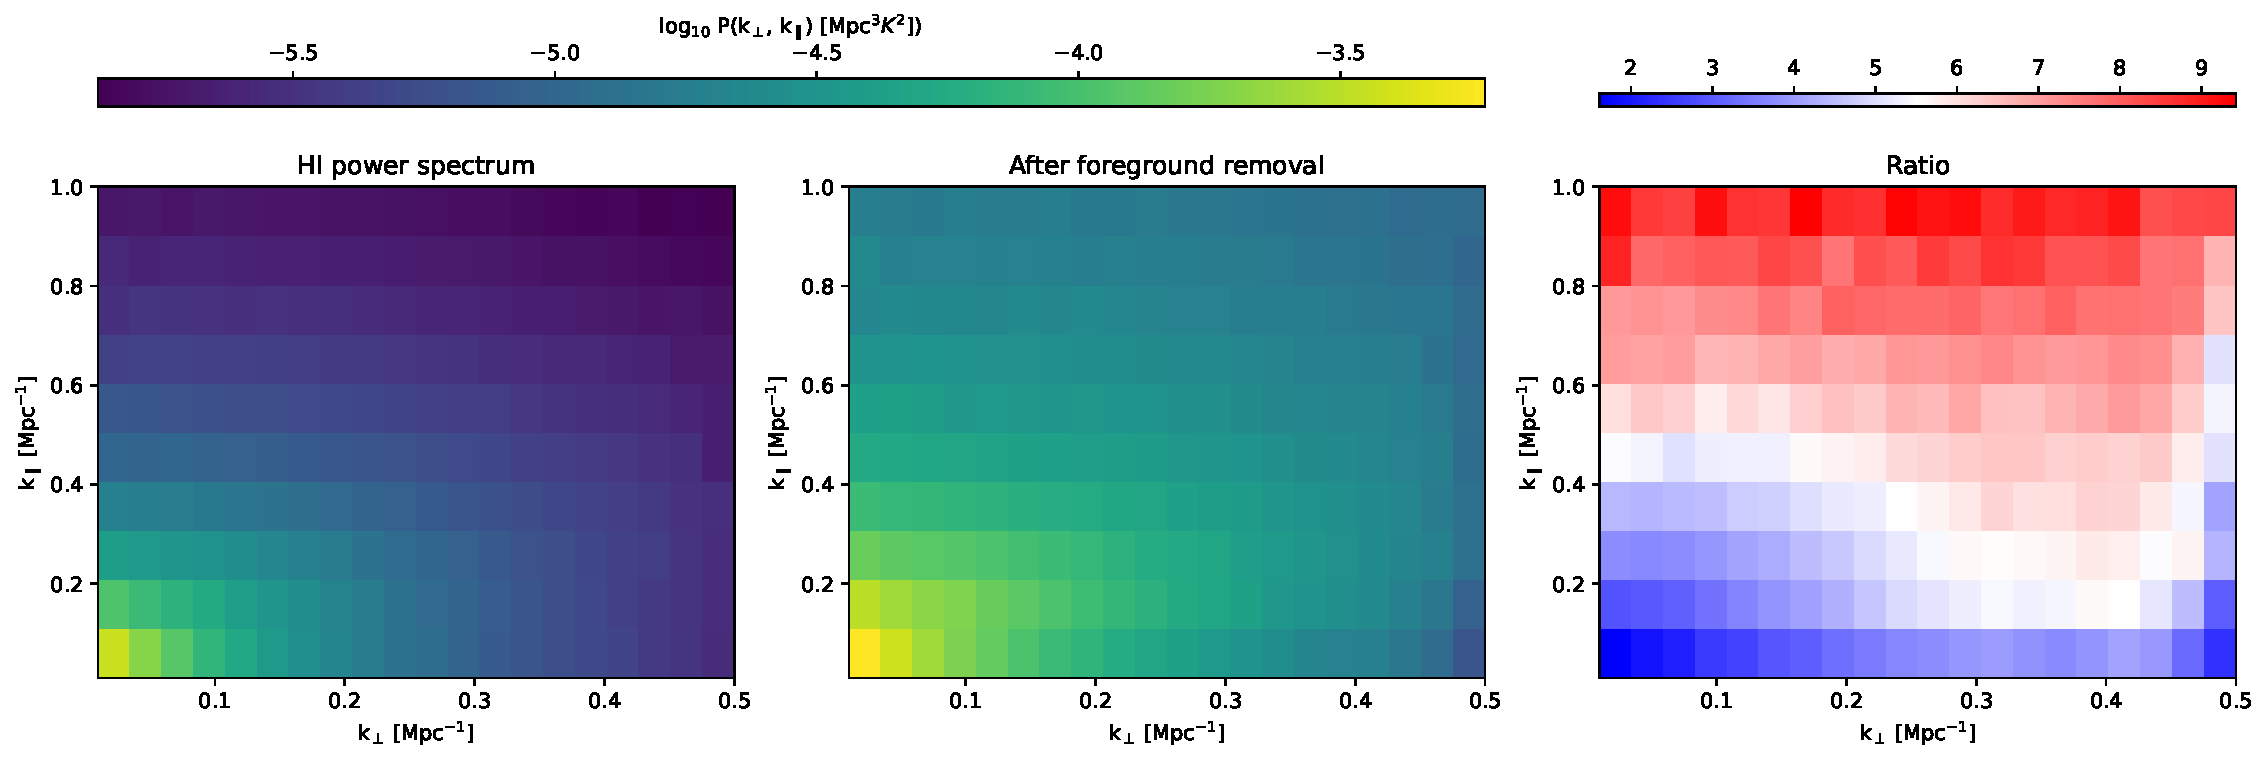
\includegraphics[width=0.9\linewidth]{outputs/week8/cylindrical_power_spectrum_fixed_l_fg_no_sp_indx.pdf}
    \caption{Enter Caption}
    \label{fig:placeholder}
\end{figure}

\clearpage

\subsubsection{Scipy optimize minimize, Nelder-Mead, Matern kernel with eta = free parameter}

\begin{figure}[htb!]
    \centering
    \begin{minipage}{0.49\textwidth}
        \centering
        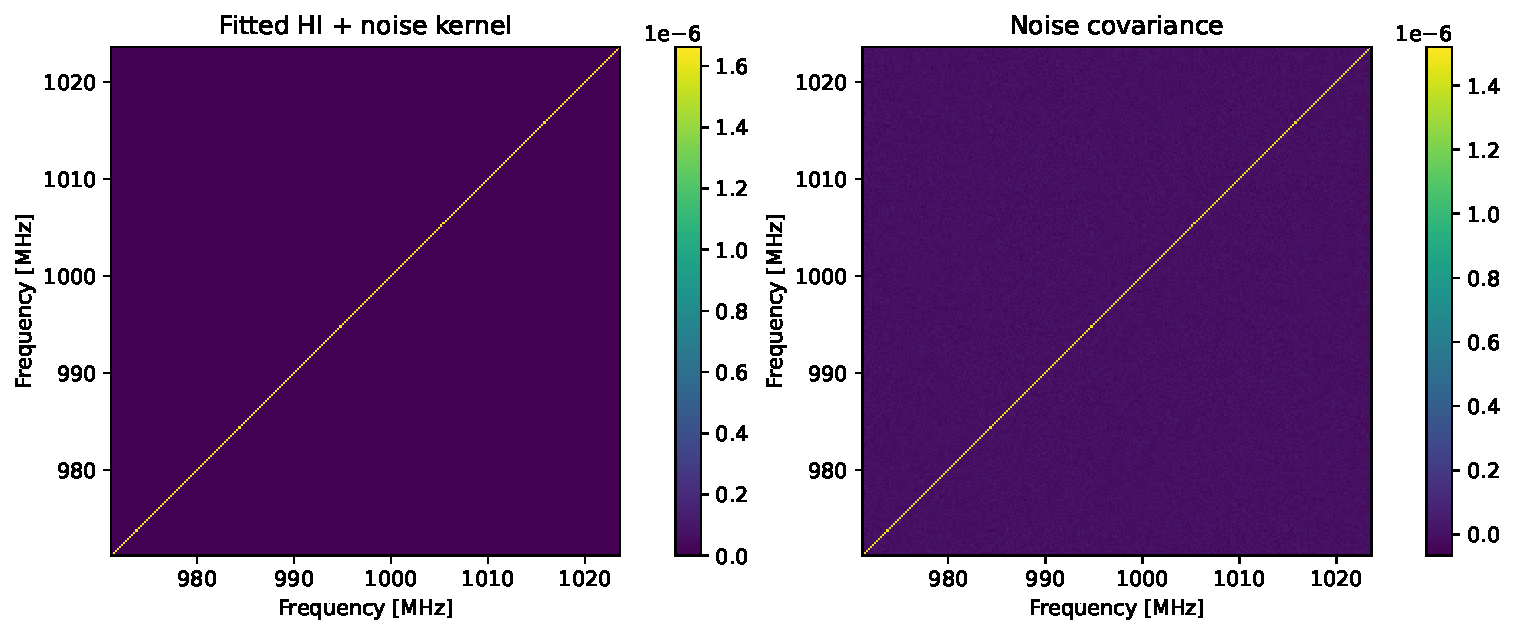
\includegraphics[width=\linewidth]{outputs/week8/hi_signal_kernal_comparison_eta_free_param_nelder_mead.pdf}
        \label{fig:pspec_lin_0_01}
    \end{minipage}
    \hfill
    \begin{minipage}{0.49\textwidth}
        \centering
        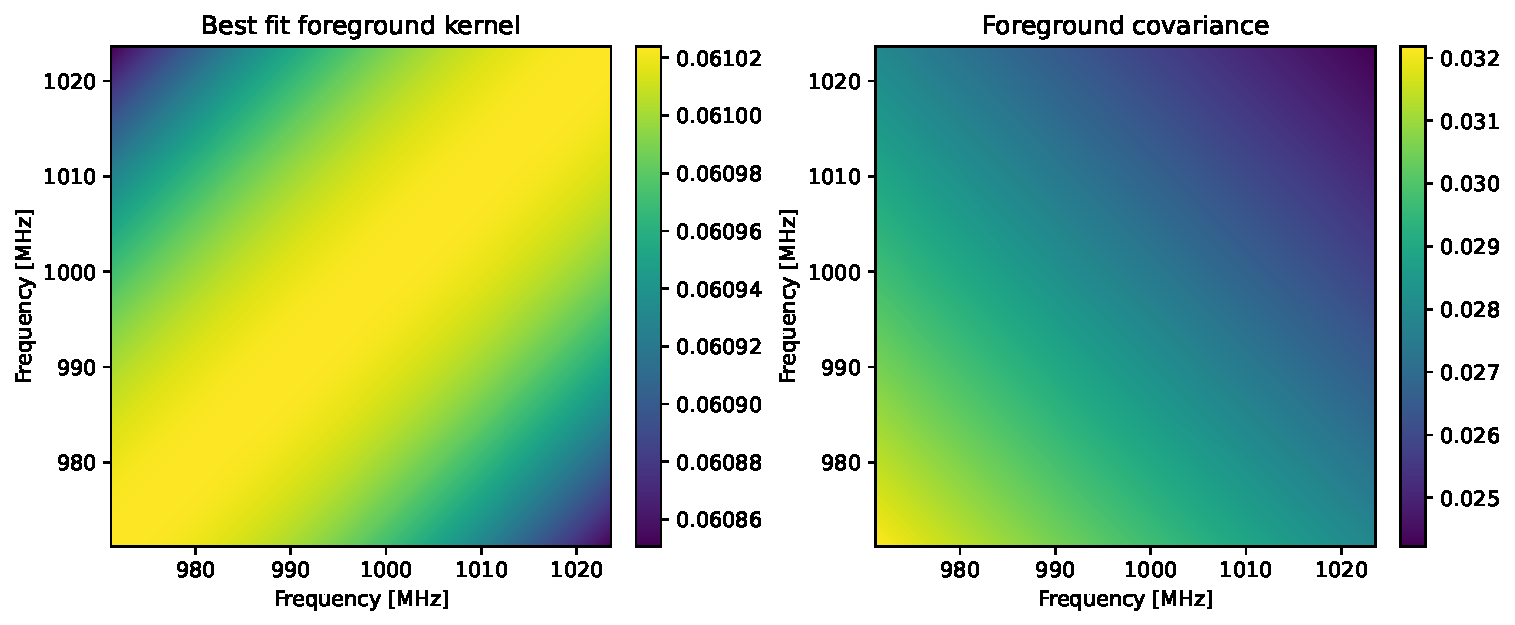
\includegraphics[width=\linewidth]{outputs/week8/fg_signal_kernal_comparison_eta_free_param_nelder_mead.pdf}
        \label{fig:pspec_log_0_01}
    \end{minipage}
    \caption{Enter Caption}
\end{figure}

\begin{figure}[hbt!]
    \centering
    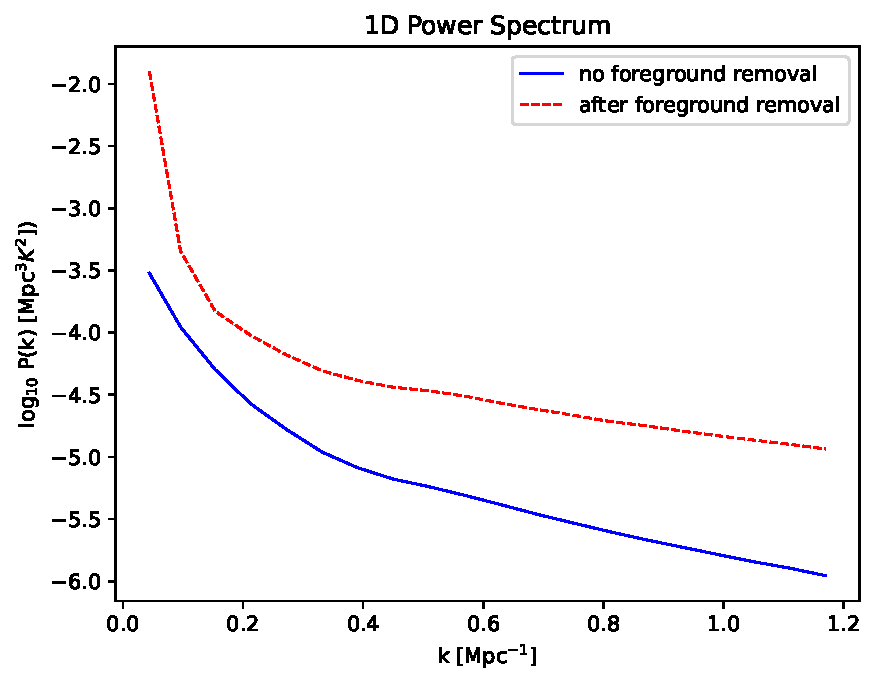
\includegraphics[width=0.4\linewidth]{outputs/week8/log_1d_power_spectrum_eta_free_param_nelder_mead.pdf}
    \caption{Enter Caption}
    \label{fig:placeholder}
\end{figure}

\begin{figure}[hbt!]
    \centering
    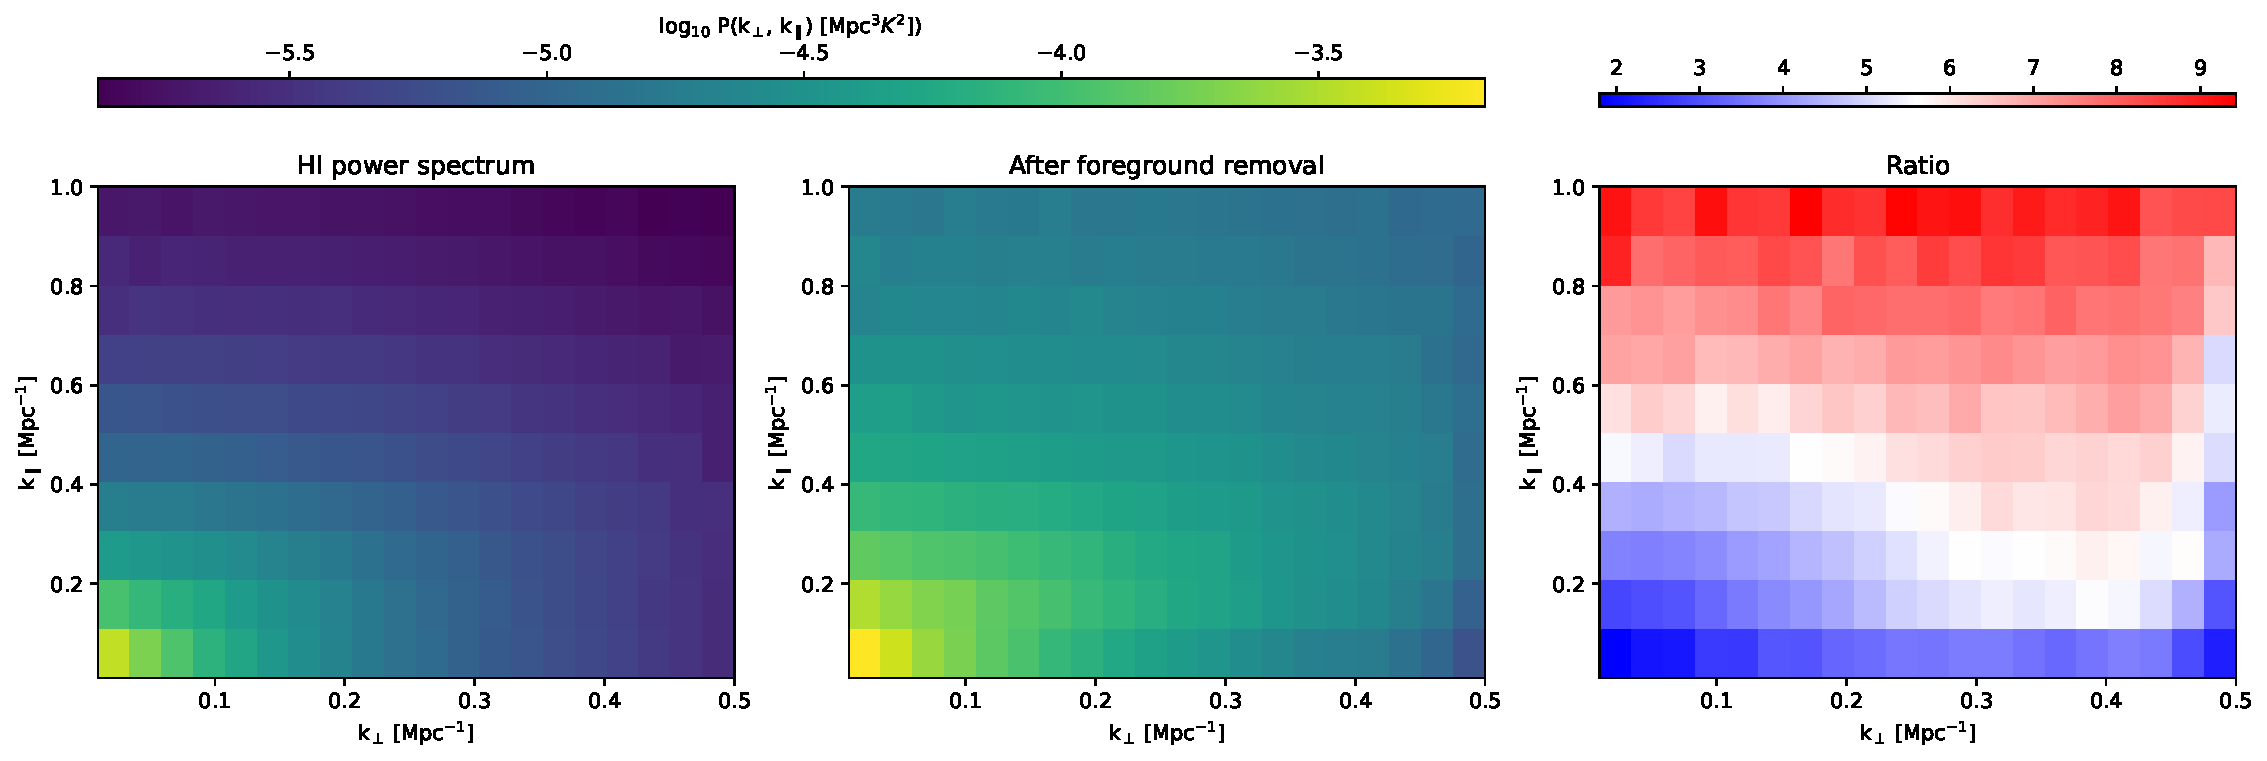
\includegraphics[width=0.9\linewidth]{outputs/week8/cylindrical_power_spectrum_eta_free_param_nelder_mead.pdf}
    \caption{Enter Caption}
    \label{fig:placeholder}
\end{figure}

\clearpage

\subsubsection{Scipy optimize minimize, Nelder-Mead, Matern kernel with eta = 5/2}

\begin{figure}[htb!]
    \centering
    \begin{minipage}{0.49\textwidth}
        \centering
        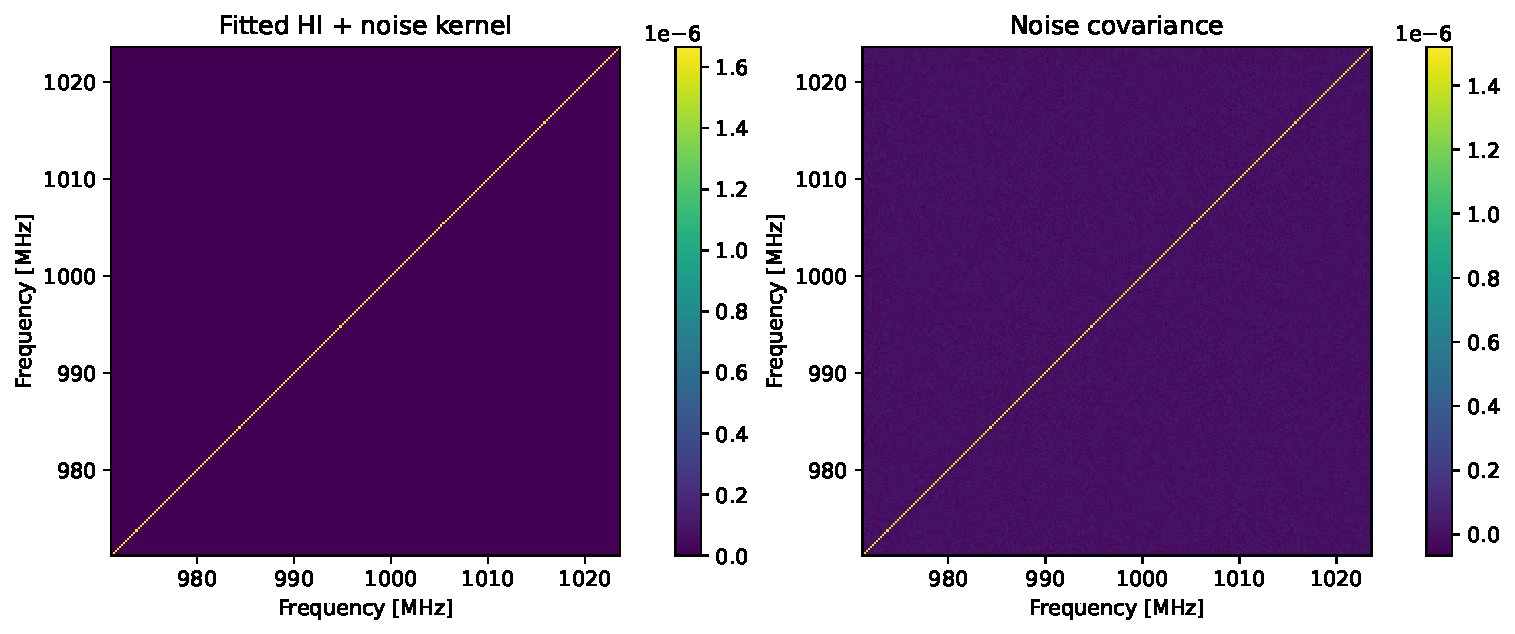
\includegraphics[width=\linewidth]{outputs/week8/hi_signal_kernal_comparison_eta_5_2_nelder_mead.pdf}
        \label{fig:pspec_lin_0_01}
    \end{minipage}
    \hfill
    \begin{minipage}{0.49\textwidth}
        \centering
        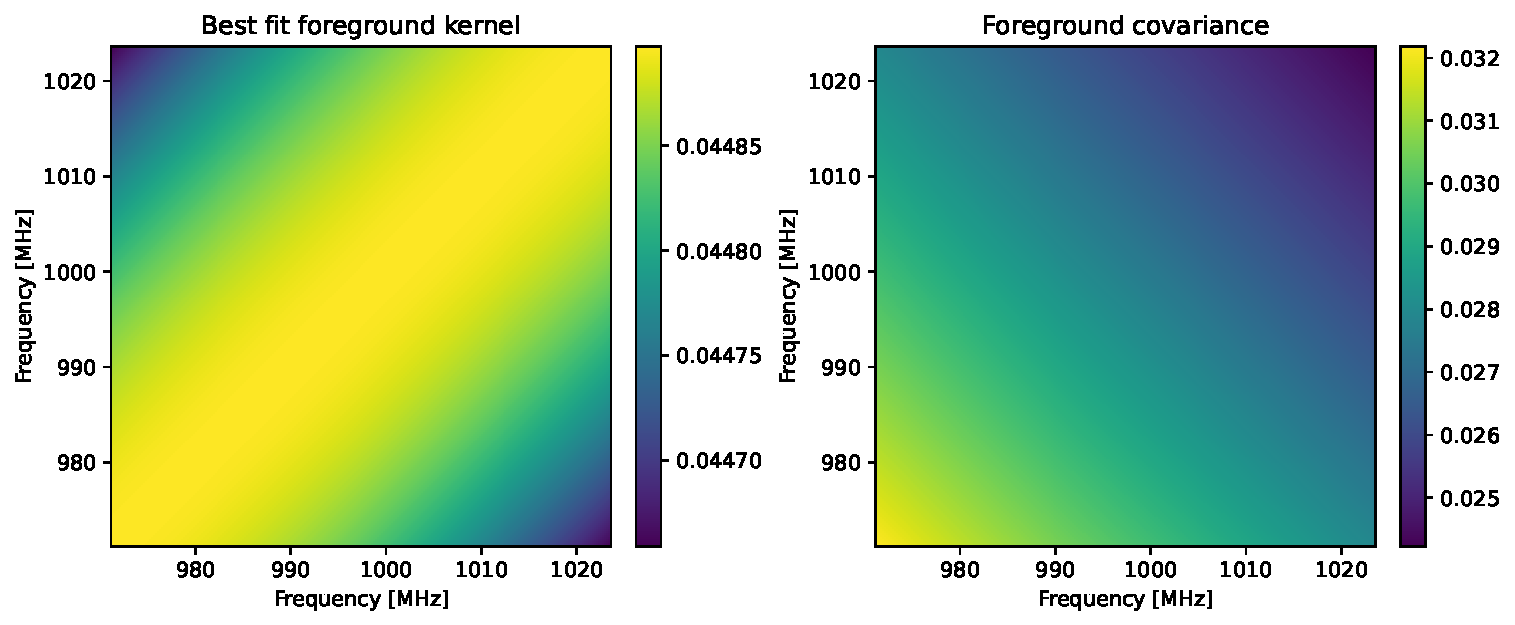
\includegraphics[width=\linewidth]{outputs/week8/fg_signal_kernal_comparison_eta_5_2_nelder_mead.pdf}
        \label{fig:pspec_log_0_01}
    \end{minipage}
    \caption{Enter Caption}
\end{figure}

\begin{figure}[hbt!]
    \centering
    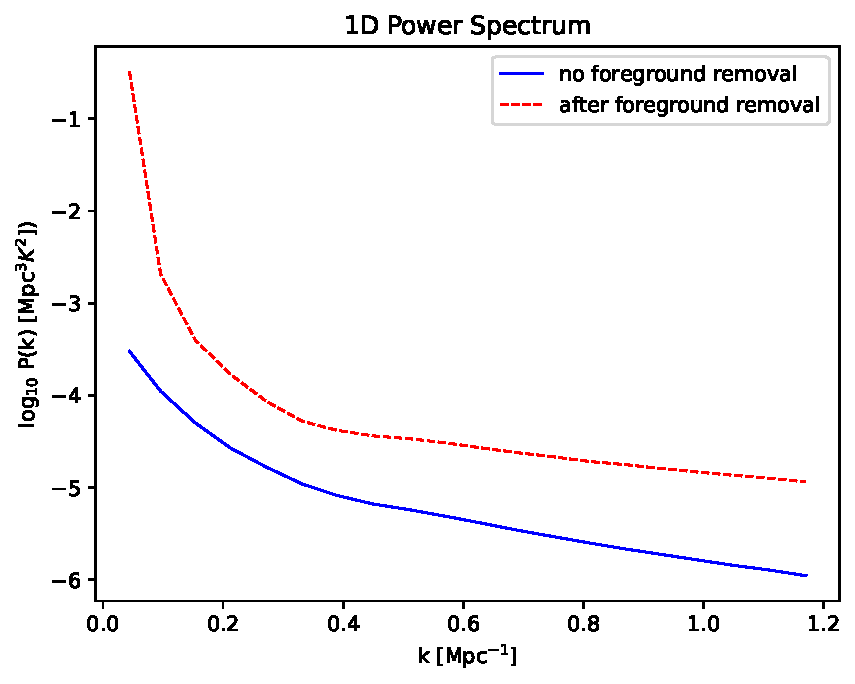
\includegraphics[width=0.4\linewidth]{outputs/week8/log_1d_power_spectrum_eta_5_2_nelder_mead.pdf}
    \caption{Enter Caption}
    \label{fig:placeholder}
\end{figure}

\begin{figure}[hbt!]
    \centering
    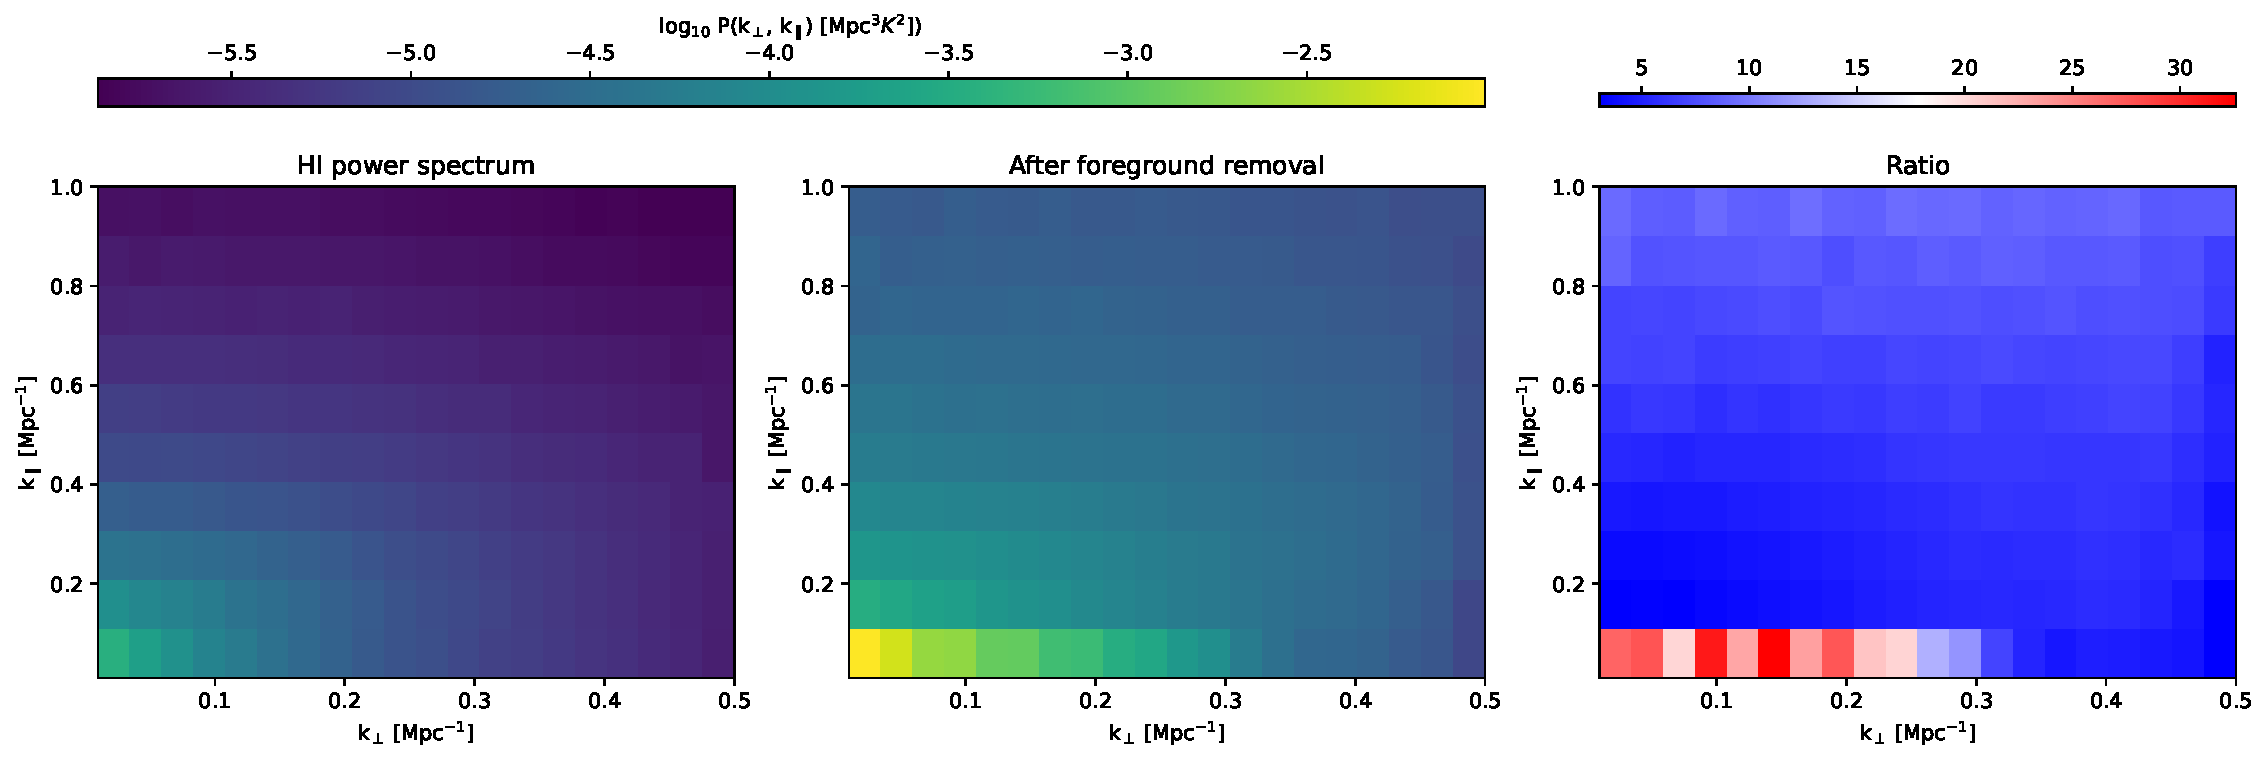
\includegraphics[width=0.9\linewidth]{outputs/week8/cylindrical_power_spectrum_eta_5_2_nelder_mead.pdf}
    \caption{Enter Caption}
    \label{fig:placeholder}
\end{figure}

\clearpage

\subsubsection{Scipy optimize minimize, Nelder-Mead, Matern kernel with eta = 3/2}

\begin{figure}[htb!]
    \centering
    \begin{minipage}{0.49\textwidth}
        \centering
        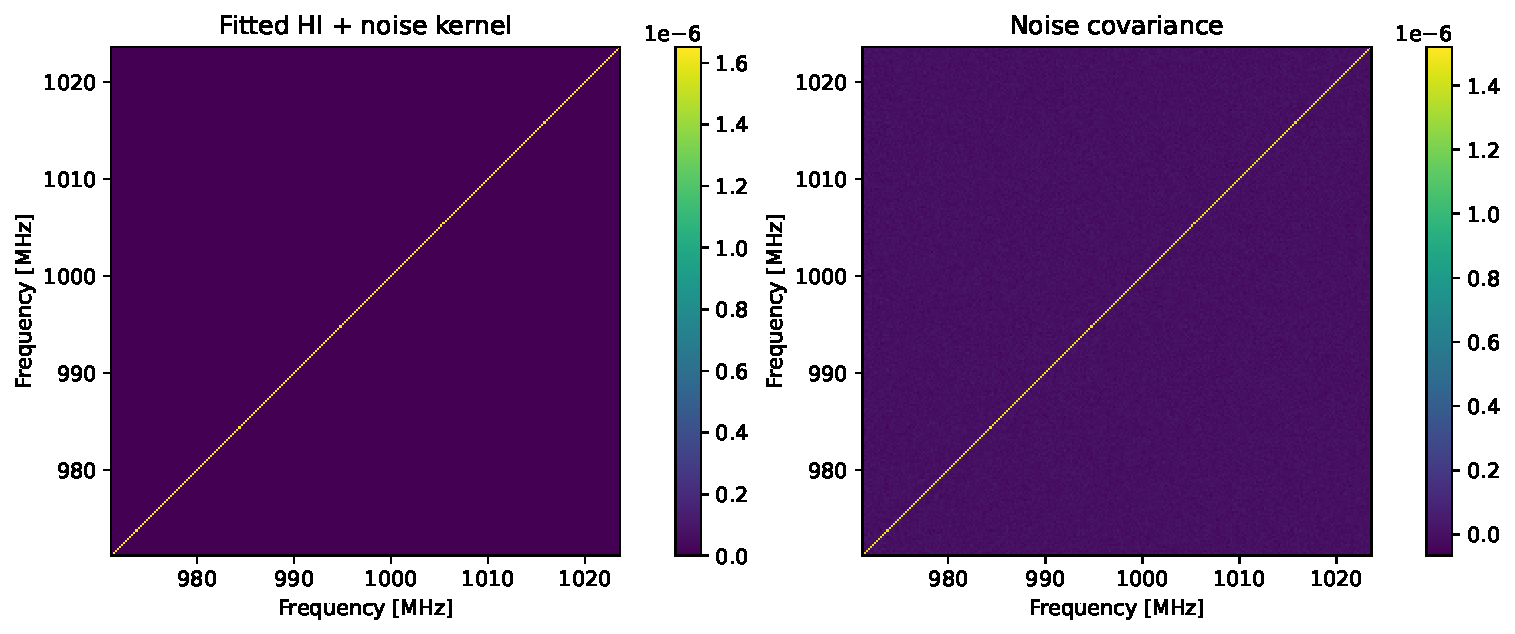
\includegraphics[width=\linewidth]{outputs/week8/hi_signal_kernal_comparison_eta_3_2_nelder_mead.pdf}
        \label{fig:pspec_lin_0_01}
    \end{minipage}
    \hfill
    \begin{minipage}{0.49\textwidth}
        \centering
        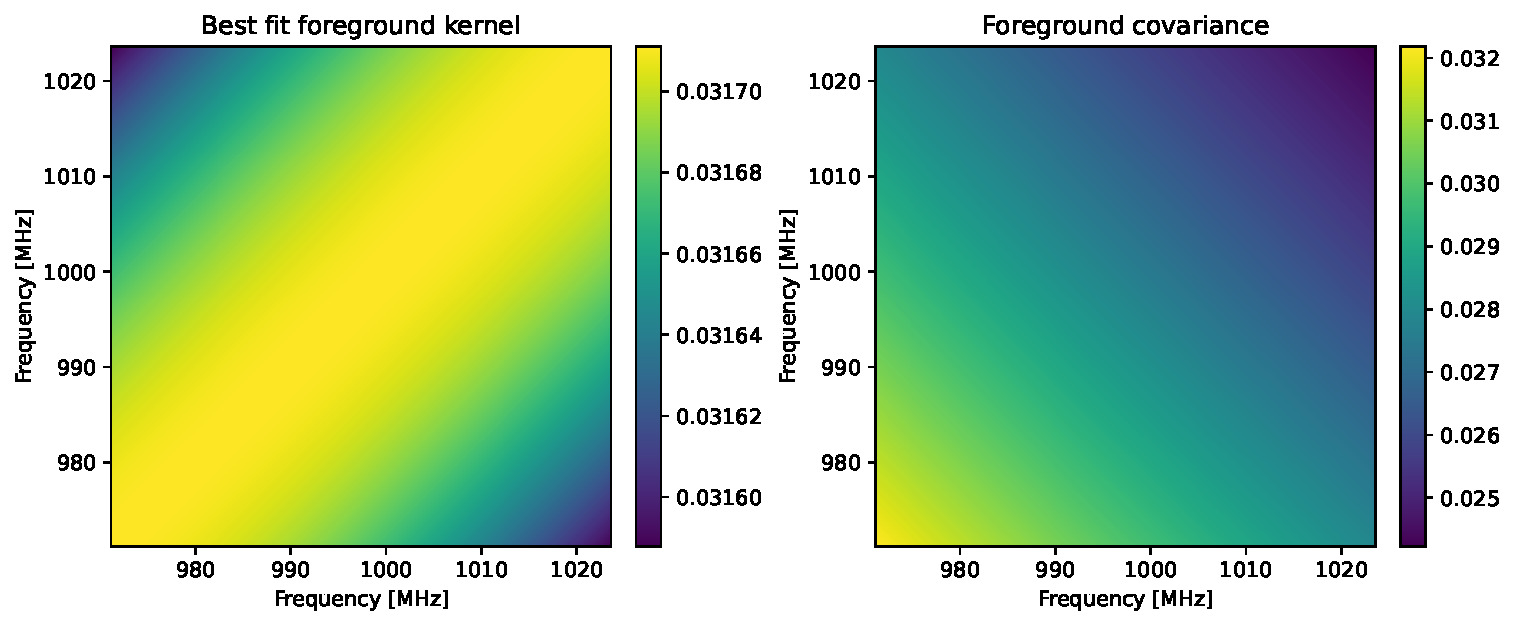
\includegraphics[width=\linewidth]{outputs/week8/fg_signal_kernal_comparison_eta_3_2_nelder_mead.pdf}
        \label{fig:pspec_log_0_01}
    \end{minipage}
    \caption{Enter Caption}
\end{figure}

\begin{figure}[hbt!]
    \centering
    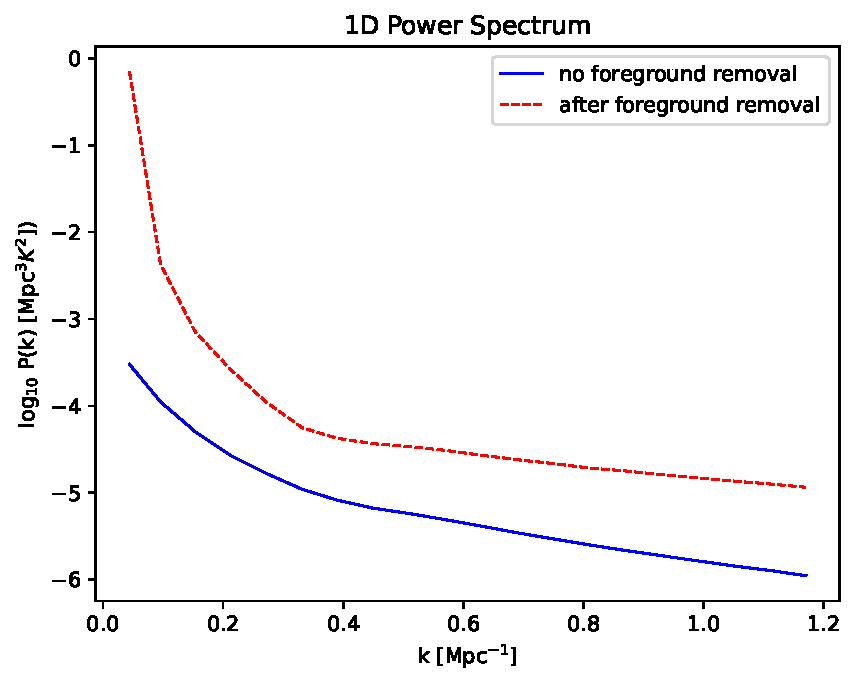
\includegraphics[width=0.4\linewidth]{outputs/week8/log_1d_power_spectrum_eta_3_2_nelder_mead.pdf}
    \caption{Enter Caption}
    \label{fig:placeholder}
\end{figure}

\begin{figure}[hbt!]
    \centering
    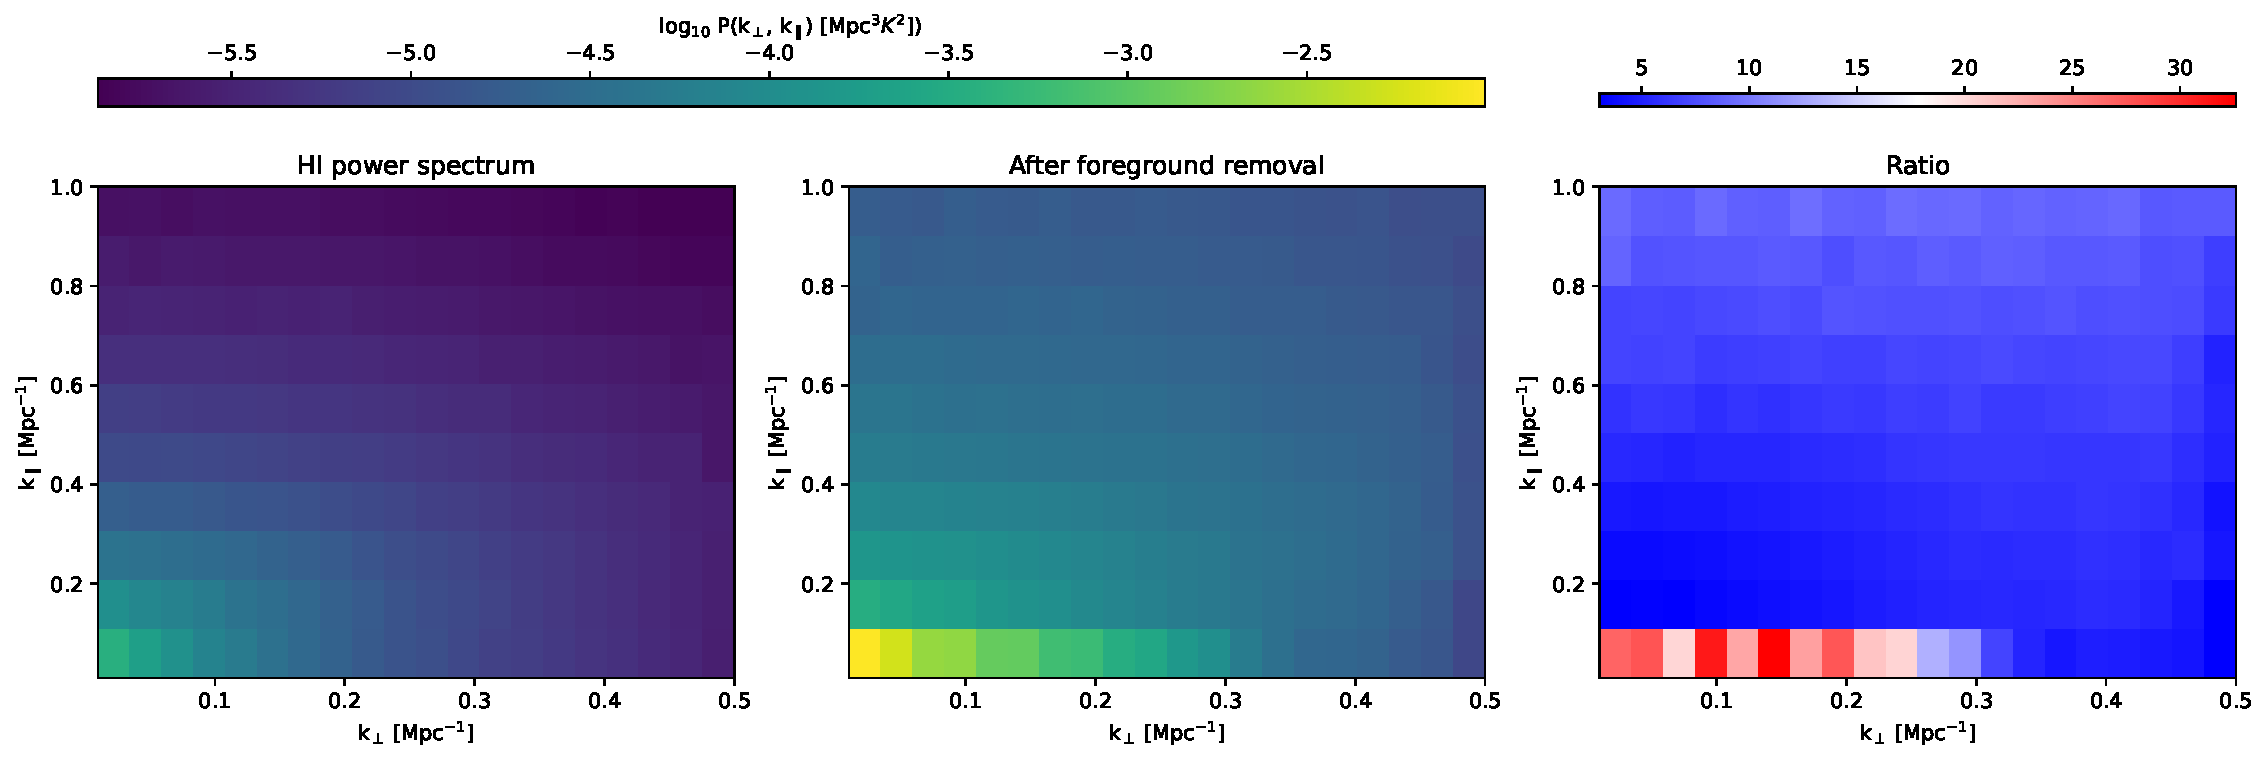
\includegraphics[width=0.9\linewidth]{outputs/week8/cylindrical_power_spectrum_eta_3_2_nelder_mead.pdf}
    \caption{Enter Caption}
    \label{fig:placeholder}
\end{figure}

\clearpage

\subsection{Wednesday 11th March}

\begin{itemize}
    \item I reran some of my GPR code and tidied up some of the plots
    \begin{itemize}
        \item Eg. I reformatted plots with colour bars so it looked a bit nicer, redid some of y-axis subtitles so they didn't repeat if they were in a row of three, for example.
    \end{itemize}
\item It is also important that I spend enough time working on my report. 
\item Today, I will focus on making the necessary changes and implementing any feedback I got from my draft 5 page report. This will include:
\begin{itemize}
    \item Combining the "foreground removal techniques" and "methodology" sections
    \item Revising the introduction to read a bit better
    \item Fixing some citations that had issues
    \item Add in a graph before cutting out low k. Eg. do not just show the final result for PCA but also include the stages and plots before the final results.
    \item Add in more explanation for the PCA results
\end{itemize}
\item Also, need to collect all of my results for GPR so far and put it into the lab book so it is easy to read and show for my meeting tomorrow.
\item Also, need to come up with a list of questions to ask in my meeting tomorrow. About my results and about anything I need to change from my draft 5 page report. Just so I have enough time to implement them and make changes before the deadline in a few weeks.
\end{itemize}

\subsection{Thursday 12th March}

\subsubsection{Meeting 8: Zhaoting and Alkistis}

\begin{itemize}
    \item We started off the meeting going over what we talked about in our last meeting since Alkistis was not there.
    \begin{itemize}
        \item We mainly reviewed my draft 5 page report.
        \item I also said that I tried different optimisation methods after optimize.fmin did not work, which mainly was optimize.minimize. This method did not really clean the signal properly.
        \item Zhaoting suggested trying different kernels.
    \end{itemize}
\item Then, I showed the work I have done since our last meeting.
\begin{itemize}
    \item I showed that I did MCMC for two cases: one with the spectral index and one without the spectral index.
    \item I did not have a chance to show any of the fits I did for the matern kernels with different eta values.
\end{itemize}
\item I was quite worried since none of the optimisation methods or different kernels I fitted were able to properly clean out the signal and it was under cleaned each time. This is likely due to a few reasons:
\begin{itemize}
    \item The signal is very idealised. If the data was a bit more realistic, the kernels might be able to identify the foreground signal better.
    \item Our data only uses a narrow frequency range. Paula's GPR paper uses a much wider frequency range and therefore has more data. This can contribute to their better cleaning of the signal.
    \item In summary, better data is needed.
\end{itemize}
\item Overall, the results I have,  even though I didn't manage to clean the signal properly, is good for the report and I can start properly writing it now.
\item In the report, the main thing I should discuss for the GPR section is the MCMC results with the corner plots. Include the cylindrical power spectrum as well, but mainly talk about the corner plots.
\begin{itemize}
    \item Make sure to discuss at length all of the steps taken to get to these final results. Eg. the priors, posteriors, burn in time, everything.
    \begin{itemize}
        \item Talk about how I tried different kernels with different eta values and eta kept on hitting the upper bounds, no matter how much I increased the bounds by, suggesting that eta = infinity, the RBF kernel, is the best fit. 
        \item Talk about how I tried to fit the RBF kernel with no spectral index and even though the length scale or whatever is fit properly, it still does not describe the signal and something is missing. The RBF kernel without the spectral index has better constrains.
        \item The RBF kernel with the spectral index is not as well constrained, specifically with the foreground parameters. The HI parameters we can see they agree and are within one sigma of each other. 
    \end{itemize}
    \item Also, discuss the results from each of the parameters and if they are or are not what we expect. 
    \begin{itemize}
        \item The HI signal is quite well constrained, as well as the spectral index. The true input values are within the sigma ranges from MCMC. 
        \item There is degeneracy between the parameters.
        \item The length scale for the foreground keep on growing. This is because as it grows, the kernel can't tell the different between a large number and infinity so it will just continue to grow. I think? I might be remembering this wrong.
        \item Also, make my corner plots look a bit nicer. There are ways to change it in the corner plot package. 
    \end{itemize}
\end{itemize}
\item I also asked about a literature review in the report.
\begin{itemize}
    \item A separate section for the literature review is not needed. However, I can and should add another paragraph second to last in the introduction (after explaining the main challenges with HI intensity mapping) to different techniques in the field which are used to address this. 
    \item When comparing to literature, just mention other papers when necessary. Eg, when discussing my results and explaining why my method is different to other methods. 
    \item Then I can go onto the final paragraph which explain what I will be using (PCA and GPR). Also, I can add in more detail about the steps I used and explain each of the sections. Don't include a table of contents page, just explain each of the sections at the end of the introduction, mimic an academic paper.
\end{itemize}
\item When writing the GPR part of the paper, write it in a similar fashion to other papers that use MCMC as their main result. Eg. have a table of the priors, results, etc. 
\item For our meeting next week, we will go over my code for MCMC and make sure it is all correct, just to double check it.
\item By our next meeting:
\begin{itemize}
    \item I want to have a complete first draft of the report, having written about everything I want to but it will not be polished. This is just because I want to make sure I fully understand everything I am writing about.
    \item Ideally, it would be close to finished but maybe that is optimistic.
    \item I want to have a set of questions to ask to clarify anything I am confused about. 
    \item I want to also have a decent understanding on MCMC and the reasons behind each step I took.
    \item I want to also have a go at the poster to get brief feedback on it.
\end{itemize}
\item Then, in the final week before the deadline, I can just do polishing of the report and the poster.
\end{itemize}